\chead[\bfseries\large SOF Olympiad Practice \\ GK: 2.Earth and its Environment]{}

\begin{document}

\begin{center}
    \fbox{\fbox{\parbox{5.5in}{\centering
    Answer all the questions.
    }}}
\end{center}

\begin{questions}

\question Study the Venn diagram. \\ X is likely to be \fillin . \\

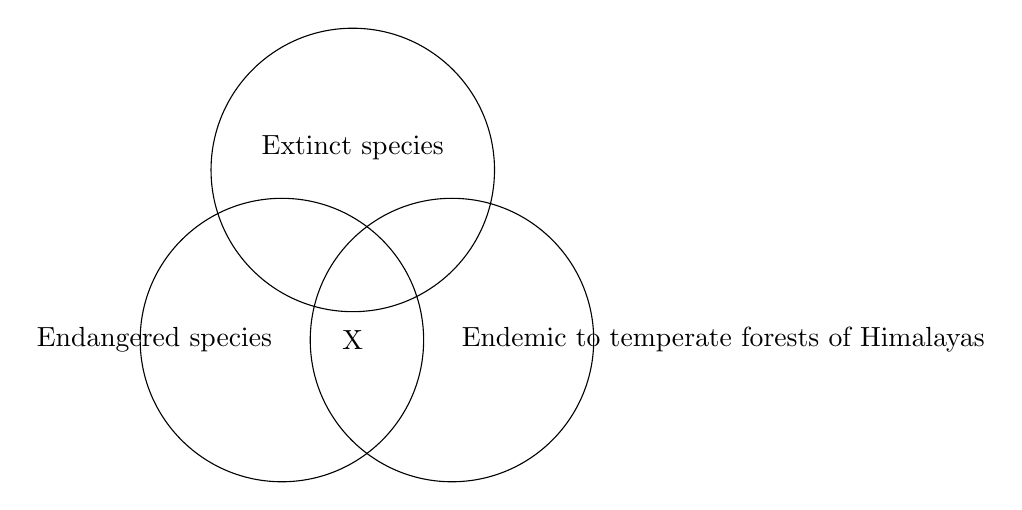
\begin{tikzpicture}
    % Define circle radii and positions
    \def\radius{1.8}
    \def\shift{1.2}

    % Draw circles
    \draw (0,0) circle (\radius) node[left] {Endangered species};
    \draw (\shift*\radius,0) circle (\radius) node[right] {Endemic to temperate forests of Himalayas};
    \draw (\radius/2,\shift*\radius) circle (\radius) node[above] {Extinct species};

    % Label the intersection
    \node at (0.5*\radius, 0.5*\radius/360) {X};
\end{tikzpicture}

\begin{randomizeoneparchoices}
    \CorrectChoice Red panda
    \choice Blackbuck
    \choice Woolly mammoth
    \choice Indian gazelle
\end{randomizeoneparchoices}

\question Project tiger was started in 1973. Its aim is to create reserves in selected areas of India to increase the tiger population. Identify which of the following is \textbf{NOT} a tiger reserve.

    \begin{choices}
        \begin{minipage}[t]{0.45\textwidth}
        \CorrectChoice Keoladeo Ghana National Park
        \choice Dudhwa National Park
    \end{minipage}
    \begin{minipage}[t]{0.45\textwidth}
        \choice Kanha National Park
        \choice Simlipal National Park
    \end{minipage}
    \end{choices}

    \question Which of the following statements is incorrect?

    \begin{randomizechoices}
        \choice Acid rain caused the weakening of Jefferson Memorial (USA) by removing silicate mineral inclusions from the marble columns of it.
        \choice Excess pumping of groundwater reduces the water table.
        \choice Ozone layer depletion increases UVB levels, which could lead to damage to human body, including skin cancer.
        \CorrectChoice Major greenhouse gases include CFCs and hydrocarbons only.
    \end{randomizechoices}

    \question The silent Valley National Park in Kerala is home to a large population of which endangered primate?

    \begin{randomizeoneparchoices}
        \CorrectChoice Lion tailed macaque
        \choice Orangutan
        \choice Chimpanzee
        \choice Gorilla
    \end{randomizeoneparchoices}

    \question Central Pollution Control Board (CPCB) initiated NAAQM programme later known as NAMP programme to check air quality in India. \\ What does NAMP stands for?

    \begin{randomizechoices}
        \CorrectChoice National Air Quality Monitoring Programme
        \choice National Air Quality Maintaining Programme
        \choice National Air Quality and Quantity Maintaining Programme
        \choice None of these
    \end{randomizechoices}

    \question Eight pollutants act as major parameters in deriving the Air Quality Index (AQI) of an area. Which of the following pollutants is not one among them?

    \begin{randomizeoneparchoices}
        \CorrectChoice Arsenic
        \choice \(\textnormal{PM}_{2.5}\)
        \choice \(\textnormal{O}_3\)
        \choice Pb
    \end{randomizeoneparchoices}

    \question Ruppell's Vulture is one of the largest vultures in the world and it also holds the record for the highest flying bird in the world. It mainly inhabits in the Sahel region of Africa. What is its current status in the IUCN Red List?

    \begin{randomizeoneparchoices}
        \CorrectChoice Critically endangered
        \choice Extinct
        \choice Least concern
        \choice Vulnerable
    \end{randomizeoneparchoices}

    \question In order to reduce land pollution from industrial operations, some methods have been developed to reduce the volume of waste. Name the method in which waste is burned in the absence of oxygen. This method also produces stable end products.

    \begin{randomizeoneparchoices}
        \CorrectChoice Pyrolysis
        \choice Shredding
        \choice Scrubbing
        \choice Electrostatic induction
    \end{randomizeoneparchoices}

    \question Match column I with column II and select the correct option from the codes given below.

    \begin{matchtabularh}
        \textbf{Column I} &  \textbf{Column II}
    \end{matchtabularh}
    
    \begin{matchtabular}
        Sulphur dioxide in air & Damage ozone layer \\ 
        CFCs & Leads to food toxicity \\ 
        Sewage dumped in river & Prevents photosynthesis \\ 
        Dust in air & Produce acid rain \\ 
        Excess fertiliser in fields & Causes water borne diseases \\
    \end{matchtabular}

    \begin{randomizechoices}
        \CorrectChoice (i)-(d), (ii)-(a), (iii)-(e), (iv)-(c), (v)-(b)
        \choice (i)-(d), (ii)-(a), (iii)-(c), (iv)-(e), (v)-(b)
        \choice (i)-(b), (ii)-(e), (iii)-(a), (iv)-(c), (v)-(d)
        \choice (i)-(c), (ii)-(b), (iii)-(e), (iv)-(d), (v)-(a)
    \end{randomizechoices}

    \question Tropical cyclones are characterised by rapidly-rotating storm systems that rotate around a low pressure centre. The cloudless core of the tropical cyclone is known as the \fillin

    \begin{randomizeoneparchoices}
        \CorrectChoice Eye
        \choice Eye Rainbow
        \choice Rainband
        \choice Eye Wall
    \end{randomizeoneparchoices}

    \fbox{\parbox{6in}{
\textbf{DIRECTION:} \emph{Read the given paragraph and answer the next two questions.}
\newline
\newline
Pachmarhi Biosphere Reserve is situated in Madhya Pradesh. The biodiversity found in it is unique as the plants and animals found in it are similar to those found in upper Himalayan peaks and lower Western Ghats. It contains two wildlife sanctuaries and one national park.
}}

\question Which of the following is \textbf{NOT} a part of Pachmarhi Biosphere Reserve?

    \begin{randomizeoneparchoices}
        \CorrectChoice Dachigam National Park
        \choice Bori Wildlife Sanctuary
        \choice Satpura National Park
        \choice Pachmarhi Wildlife Sanctuary
    \end{randomizeoneparchoices}

    \question Which of the following animals are endemic to Pachmarhi Biosphere Reserve area?

    \begin{choices}
        \choice Indian giant squirrel
        \choice Flying squirrel
        \choice Bison
        \CorrectChoice All of these
    \end{choices}

    \question Riya visited her village after 10 years and found that there is a problem of desertification. What could be the probable reasons for this?
    \begin{enumerate}[align=left,label=\roman*.]
        \item Overgrazing
        \item Indiscriminate cutting of trees
        \item Poorly drained irrigation systems
    \end{enumerate}
    \begin{randomizeoneparchoices}
        \CorrectChoice (i), (ii) and (iii)
        \choice (i) and (ii) only
        \choice (ii) and (iii) only
        \choice (i) and (iii) only
    \end{randomizeoneparchoices}

    \question Area reserved for conservation of both plants and animals where grazing is not allowed is known as X while an area reserved for conservation of wild animals only is known as Y. \\ What can be placed in X and Y?

    \begin{randomizechoices}
        \CorrectChoice X \textendash National Park, Y \textendash Wildlife Sanctuary
        \choice X \textendash Wildlife Sanctuary, Y \textendash Biosphere Reserve
        \choice X \textendash National Park, Y \textendash Biosphere Reserve
        \choice X \textendash Biosphere Reserve, Y \textendash National Park
    \end{randomizechoices}

    \question Which of the following is a floating National Park situated in India?

    \begin{randomizeoneparchoices}
        \CorrectChoice Keibul Lamjao National Park
        \choice Manas National Park
        \choice Mollem National Park
        \choice Betla National Park
    \end{randomizeoneparchoices}

    \question The elimination of this pest under the Four Pests Campaign of China that was initiated in 1958 upset the ecological balance and enabled crop-eating insects to proliferate. Identify the pest.

    \begin{randomizeoneparchoices}
        \CorrectChoice Sparrow
        \choice Bees
        \choice Beetles
        \choice Locust
    \end{randomizeoneparchoices}

    \question Which of the following is a constituent of automobile exhaust?

    \begin{choices}
        \choice Carbon monoxide
        \choice Carbon dioxide
        \choice Nitrogen oxides
        \CorrectChoice All of these
    \end{choices}

    \question The common house sparrow population has been declining in many Asian countries especially in India. To promote its conservation which state's Chief Minister had declared it as the state bird?

    \begin{randomizeoneparchoices}
        \CorrectChoice Delhi
        \choice Tamil Nadu
        \choice West Bengal
        \choice Goa
    \end{randomizeoneparchoices}

    \question Read the following statements and select the correct ones.
    \begin{enumerate}[align=left,label=\roman*.]
        \item Biodiversity hotspots are those specific regions which have large number of endemic species.
        \item The passenger pigeon is an extinct bird.
        \item The term ecology was coined by Enst Haeckel in 1866.
        \item Gandhi Peace Prize was awarded to a noted environmentalist Chandi Prasad Bhatt in 2013.
    \end{enumerate}
    \begin{randomizeoneparchoices}
        \CorrectChoice (i), (ii), (iii) and (iv)
        \choice (i) and (ii) only
        \choice (i) and (iv) only
        \choice (ii) and (iii) only
    \end{randomizeoneparchoices}

    \question The marble panels of Acropolis of Athens have been chemically transformed by acid rain into soft gypsum. What is the main cause of acid rain in this area?

    \begin{randomizechoices}
        \CorrectChoice Economic expansion and heavy vehicle emissions
        \choice Pollution generated by local boundaries and oil refineries
        \choice Pollution emanating from unbrindled development in the region
        \choice Pollution generated by local mining and petrochemical industries
    \end{randomizechoices}

    \question What are the sources of toxic wastes in marine life?

    \begin{choices}
        \choice Metals from mining
        \choice Industries
        \choice Insecticides and pesticides from farms
        \CorrectChoice All of these
    \end{choices}

    \question Permafrost, a permanently frozen soil, found at high altitudes is melting due to global warming. Which of the following gases are released from its melting?

    \begin{randomizeoneparchoices}
        \CorrectChoice Carbon dioxide and methane
        \choice Ozone and methane
        \choice Hydrogen and ozone
        \choice Nitrogen oxide and hydrogen
    \end{randomizeoneparchoices}

    \question The given picture of tall and thin blades of hardened snow are believed to be formed by strong winds of Andes mountains. This type of snow formation in high altitudes is known as \fillin

    \begin{figure}[h!]
        \centering
        \includegraphics[width=3cm]{02_penitentes.jpg}
      \end{figure}

    \begin{randomizeoneparchoices}
        \CorrectChoice Penitentes
        \choice Ice circles
        \choice Pointing stones
        \choice Moving stones
    \end{randomizeoneparchoices}

    \question Match column I with column II and select the correct option from the given codes.

    \begin{matchtabularh}
        \textbf{Column I} &  \textbf{Column II}
    \end{matchtabularh}
    
    \begin{matchtabular}
        Okapi Wildlife Reserve & New Caledonia rainforest \\ 
        Biosphere Reserve Srilanka & Ituri rainforest \\ 
        Kagu, an endangered bird & Hawaiian rainforest \\ 
        Top canopy dominated by \emph{Acacia koa} & Sinharaja rainforest \\ 
    \end{matchtabular}

    \begin{randomizechoices}
        \CorrectChoice (i)-(b), (ii)-(d), (iii)-(a), (iv)-(c)
        \choice (i)-(a), (ii)-(c), (iii)-(b), (iv)-(d)
        \choice (i)-(b), (ii)-(a), (iii)-(c), (iv)-(d)
        \choice (i)-(c), (ii)-(b), (iii)-(d), (iv)-(a)
    \end{randomizechoices}

    \question A rainforest is a huge dense lush forest having four distinct layers. Which of the following layers lies above the canopy layer?

    \begin{randomizeoneparchoices}
        \CorrectChoice Emergent
        \choice Forest floor
        \choice Understorey
        \choice Canopy is the uppermost layer
    \end{randomizeoneparchoices}

\end{questions}


\end{document}